\documentclass[aspectratio=169,10pt]{beamer}
\usepackage{graphicx,booktabs,tikz,pgfplots}
\pgfplotsset{compat=1.16}
\usepackage{beamer_iiti}
\AtBeginSection[]{}
\graphicspath{{figures/}}
\colorlet{accent}{iiticyan}
\colorlet{navy}{iitiblue}
\setbeamersize{text margin left=7mm,text margin right=7mm}
\newcommand{\flowpoint}[1]{\par\noindent\hangindent=1em\hangafter=1\makebox[1em][l]{\textcolor{iitiblue}{\textbullet}}#1\par}
\newcommand{\key}[1]{\par\smallskip{\color{iitiblue}\bfseries #1}\par}
\newcommand{\pair}[3]{\begin{columns}[c,onlytextwidth]
\begin{column}{.55\textwidth}\centering\includegraphics[width=\linewidth,height=4.65cm,keepaspectratio]{#1}\end{column}
\begin{column}{.42\textwidth}\begin{block}{#2}\small #3\end{block}\end{column}\end{columns}}
\title[Financial Market Forecasting and Algorithmic Trading]{Machine Learning for Financial Market Forecasting and Algorithmic Trading}
\subtitle{B.Tech Project Final Presentation}
\author[Prince Kumar]{\textbf{Prince Kumar} (Roll No. 230051013)\\[.5em]\small\textbf{Supervisors:} Prof. Raghunath Sahoo and Dr. Kalindi C. Pradhan}
\institute[IIT Indore]{Engineering Physics, Department of Physics\\\textbf{Indian Institute of Technology Indore}}
\date{}
\begin{document}
\begin{withoutheadline}
\begin{frame}[plain]\titlepage\note{\textbf{0:00 to 0:16}\par Suppose I correctly predict tomorrow's exchange-rate direction. Have I found a profitable trade? I set out to test that question in two stages: forecasting daily currencies, then trading intraday equities under capital limits and fees.}
\end{frame}
\end{withoutheadline}
\section{Overview}
\subsection*{}
\begin{frame}{Why I started with forecasting}
\centering
\begin{tikzpicture}[card/.style={draw=iitiblue!40,fill=iitilightbg,rounded corners=2pt,text width=6.45cm,minimum height=2.28cm,align=left,inner sep=4pt,font=\small},route/.style={->,>=stealth,thick,draw=iiticyan}]
\node[card] (s0) at (0,0) {\textcolor{iitiblue}{\bfseries 1. I began with the literature}\par\smallskip \flowpoint{I reviewed how researchers forecast exchange rates.} \flowpoint{Deep learning interested me because it could learn interactions between currencies and interest rates.}};
\node[card] (s1) at (7.3,0) {\textcolor{iitiblue}{\bfseries 2. I needed a simple benchmark}\par\smallskip \flowpoint{I tried three baselines: today's price as tomorrow's forecast, a moving average and ARIMA.} \flowpoint{I used them to judge whether a network improved the forecast.}};
\node[card] (s2) at (7.3,-2.77) {\textcolor{iitiblue}{\bfseries 3. I expanded the inputs in stages}\par\smallskip \flowpoint{I began with five currency and interest-rate inputs.} \flowpoint{Adding 18 technical indicators gave me 23 inputs.} \flowpoint{Adding five days of lags brought the total to 138.}};
\node[card] (s3) at (0,-2.77) {\textcolor{iitiblue}{\bfseries 4. I tested how the model used history}\par\smallskip \flowpoint{I trained the early networks with Adam and mean squared error.} \flowpoint{My daily forex LSTM used ten days, 32 hidden units and a linear output.} \flowpoint{For NIFTY, I also tested a bidirectional LSTM.}};
\draw[route] (s0.east)--(s1.west);\draw[route] (s1.south)--(s2.north);\draw[route] (s2.west)--(s3.east);
\end{tikzpicture}
\note{\textbf{0:16 to 0:54}\par I wanted to know what deep learning could add beyond simple forecasts. I built the baselines first, then added market, technical and lagged inputs. In the forex LSTM, ten daily observations produced one next-day return forecast.}
\end{frame}
\begin{frame}{Why I changed the loss and simulated trades}
\centering
\begin{tikzpicture}[card/.style={draw=iitiblue!40,fill=iitilightbg,rounded corners=2pt,text width=6.45cm,minimum height=2.28cm,align=left,inner sep=4pt,font=\small},route/.style={->,>=stealth,thick,draw=iiticyan}]
\node[card] (s0) at (0,0) {\textcolor{iitiblue}{\bfseries 5. More data gave me a puzzle}\par\smallskip \flowpoint{I added gold, crude oil and World Bank Pink Sheet commodity prices.} \flowpoint{Forecasts often stayed close to zero.} \flowpoint{I suspected gaps and noise in the data. Their individual effects remain untested.}};
\node[card] (s1) at (7.3,0) {\textcolor{iitiblue}{\bfseries 6. A small error could hide a weak forecast}\par\smallskip \flowpoint{Many daily returns clustered around zero.} \flowpoint{Predicting almost no change could yield a small squared error even when the model missed a large move.}};
\node[card] (s2) at (7.3,-2.77) {\textcolor{iitiblue}{\bfseries 7. I changed what training emphasized}\par\smallskip \flowpoint{I gave errors on larger realized moves more weight and added a penalty for the wrong sign.} \flowpoint{The weighting supplies the useful gradient. Its impact still needs a controlled comparison.}};
\node[card] (s3) at (0,-2.77) {\textcolor{iitiblue}{\bfseries 8. I put the forecast through execution}\par\smallskip \flowpoint{I simulated EUR/USD entries, exits and position sizes over 65 sessions in 2026.} \flowpoint{USD 10,000 grew to USD 10,228.30.} \flowpoint{The gain was 2.28\% over the period, or 9.15\% annualized as reported.}};
\draw[route] (s0.east)--(s1.west);\draw[route] (s1.south)--(s2.north);\draw[route] (s2.west)--(s3.east);
\end{tikzpicture}
\note{\textbf{0:54 to 1:32}\par I tried adding commodity data, yet the forecasts clustered near zero. That pushed me to change the training objective and then ask whether a forecast could survive execution. The EUR/USD simulation gained 2.28 percent over 65 sessions.}
\end{frame}
\begin{frame}{Why I moved from forecasts to trading rules}
\centering
\begin{tikzpicture}[card/.style={draw=iitiblue!40,fill=iitilightbg,rounded corners=2pt,text width=6.45cm,minimum height=2.28cm,align=left,inner sep=4pt,font=\small},route/.style={->,>=stealth,thick,draw=iiticyan}]
\node[card] (s0) at (0,0) {\textcolor{iitiblue}{\bfseries 9. I wanted to explain each trade}\par\smallskip \flowpoint{The neural model gave me a forecast, but I wanted to explain why each trade opened.} \flowpoint{I turned to rules with explicit entry conditions, stops and profit targets.}};
\node[card] (s1) at (7.3,0) {\textcolor{iitiblue}{\bfseries 10. I searched for rules and settings}\par\smallskip \flowpoint{For forex, I used a genetic algorithm to evolve numerical settings.} \flowpoint{For equities, I used grid search on four rule families and genetic programming to evolve readable entry conditions.}};
\node[card] (s2) at (7.3,-2.77) {\textcolor{iitiblue}{\bfseries 11. I tested one shared portfolio}\par\smallskip \flowpoint{I ranked stocks, shared cash across positions and charged fees. Cumulative backtest returns were:} \flowpoint{India top 10: 250.87\% vs. 220.97\% for holding.} \flowpoint{US top 20: 12.50\% vs. 40.97\% for holding.}};
\node[card] (s3) at (0,-2.77) {\textcolor{iitiblue}{\bfseries 12. RL agent}\par\smallskip \flowpoint{I gave the agent rule signals and one shared account.} \flowpoint{The US test gained 4.02\%. The agent mainly bought at the open and held until near the close.}};
\draw[route] (s0.east)--(s1.west);\draw[route] (s1.south)--(s2.north);\draw[route] (s2.west)--(s3.east);
\end{tikzpicture}
\note{\textbf{1:32 to 2:12}\par I wanted to inspect why trades happened, so I moved to readable rules and then tested them in a shared account. The Indian top ten beat holding, whereas the US top twenty trailed. The RL agent is the next experiment, and its dependence on the signals is still an open question.}
\end{frame}


\begin{frame}{When does a forecast become a profitable trade?}
\begin{columns}[T,onlytextwidth]
\begin{column}{.47\textwidth}
\key{Daily forex}
\textbf{Can a currency forecast guide a trade?}
\begin{enumerate}
\item Predict the next day's exchange rate or return.
\item Compare direction calls with always predicting up.
\item Trade EUR/USD and compare the account with holding euros.
\end{enumerate}
\end{column}
\begin{column}{.47\textwidth}
\key{Intraday equities}
\textbf{Which signals earn a place in a shared portfolio?}
\begin{enumerate}
\item Audit minute bars and test forecast-driven entries.
\item Search for trading rules and evaluate them on later months.
\item Allocate capital across stocks and measure returns after fees.
\end{enumerate}
\end{column}
\end{columns}
\note{\textbf{2:12 to 2:24}\par For forex, my first benchmark is almost embarrassingly simple: what happens if I predict up every day? For equities, the benchmark changes: could I have earned more just by holding the stocks? I use both because a good forecast and a good allocation answer different questions.}
\end{frame}

\begin{frame}{Which data sources did we use, and why?}
\small
\begin{tabular}{@{}p{.30\linewidth}@{\hspace{.025\linewidth}}p{.65\linewidth}@{}}
\toprule
\textbf{Source} & \textbf{Role in the experiments}\\\midrule
FRED & Long daily histories of exchange rates, the US policy rate and Treasury yields for forex forecasting.\\[2pt]
Yahoo Finance (\texttt{yfinance}) & Recent FX quotes and intraday EUR/USD bars for the execution simulation.\\[2pt]
Kaggle + FYERS API & Kaggle supplied historical Indian equity bars. FYERS extended coverage with recent observations (100 stock files).\\[2pt]
HF Data Library (IEX HIST) & Trade-based, one-minute bars from a named US exchange for the 95-stock replay.\\[2pt]
Nifty Indices; World Bank & Daily NIFTY 50 history for index tests; Pink Sheet commodity prices for exploratory forex inputs.\\
\bottomrule
\end{tabular}
\note{\textbf{2:24 to 2:46}\par FRED supplied long daily histories for forex and interest rates. Yahoo Finance supplied recent FX bars. For equities I needed minute-level histories across stocks: Kaggle plus FYERS for India, and IEX trade-based data through the HF Data Library for the US. The two universes contain 100 and 95 stock files, with different start dates.}
\end{frame}

\begin{frame}{What are the limitations of the Yahoo Finance data?}
\small
\begin{block}{Why qualify the Yahoo data?}
\footnotesize The \href{https://github.com/ranaroussi/yfinance/blob/main/doc/source/advanced/price_repair.rst}{\textcolor{iiticyan}{\texttt{yfinance} maintainers}} document 100-fold price errors and incorrect split or dividend adjustments in some equity histories. In our FX replay, a separate limitation is that coarse bars carried onto a minute grid cannot reveal the true intraminute price path.
\end{block}
\note{\textbf{2:46 to 2:56}\par The limitation that matters most for this replay is resolution. Carrying a five-minute or hourly observation onto a minute grid gives it a new timestamp. It tells me nothing about the order in which prices moved inside that interval.}
\end{frame}

\section{Daily forex}
\subsection*{}
\begin{frame}{USD/INR price errors fell as features were added}
\centering
\begin{tabular}{lrrr}\toprule
Model & Test days & RMSE (INR per USD) & Direction\\\midrule
Base MLP & 690 & 1.9150 & 44.93\%\\
With technical features & 680 & 0.2553 & 52.21\%\\
Technical + temporal features & 675 & 0.2395 & 52.30\%\\\bottomrule
\end{tabular}
\par\bigskip\raggedright Adding temporal features reduced RMSE again, while directional accuracy moved only 0.09 percentage points. The three runs cover slightly different test samples.
\key{The technical models predict a log return and convert it to a price for scoring.}
\note{\textbf{2:56 to 3:21}\par Follow the RMSE column downward: from about 1.92 rupees per dollar to 0.26 with technical features and 0.24 with time features. The test samples differ slightly. Smaller price errors were encouraging, but the direction score barely moved in the last step. That is why I next predicted the return directly.}
\end{frame}


\begin{frame}{Inside the USD/INR multilayer perceptron (MLP)}
\centering
\begin{tikzpicture}[x=2.85cm,y=.49cm,unit/.style={circle,draw=iitiblue,fill=iiticyan!12,minimum size=8pt,inner sep=0pt},font=\footnotesize]
\foreach \x/\lbl in {0/Inputs,1/64 neurons,2/32 neurons,3/1 output}
  \node[text=iitiblue,font=\bfseries\footnotesize] at (\x,1.9) {\lbl};
\foreach \x in {0,1,2}
  \foreach \j/\y in {1/1,2/0,3/-1} {\node[unit] (n\x\j) at (\x,\y) {};}
\node[unit] (out) at (3,0) {};
\foreach \j in {1,2,3} {\foreach \k in {1,2,3} {
  \draw[iitiblue!40] (n0\j)--(n1\k);
  \draw[iitiblue!40] (n1\j)--(n2\k);}
  \draw[iitiblue!40] (n2\j)--(out);}
\node at (1,-1.85) {ReLU};\node at (2,-1.85) {ReLU};\node at (3,-1.85) {Linear};
\end{tikzpicture}\par
{\scriptsize Representative neurons shown. Each hidden neuron computes $\max(0,\sum_i w_i x_i+b)$.}\par\smallskip
\small
\begin{tabular}{@{}lcr@{}}\toprule
USD/INR model & Input features & Weights + biases\\\midrule
Base & 5 market inputs & 2,497\\
Technical & 5 market + 18 indicators & 3,649\\
Technical + temporal & 23 features $\times$ (today + 5 lags) = 138 & 11,009\\\bottomrule
\end{tabular}\par\smallskip
\raggedright\footnotesize The temporal model adds 20\% dropout after each ReLU during training. The base model predicts price; both technical models predict next-day log return.
\note{\textbf{3:21 to 3:53}\par Read the network from left to right. Each circle combines its inputs using learned weights and a bias; ReLU passes positive values forward. All three models have two hidden layers, with 64 and 32 neurons. We added features and then five days of lags, expanding the input from five to 23 to 138. The temporal model also drops 20 percent of hidden activations during training. Its 11,009 trainable parameters include weights and biases.}
\end{frame}

\begin{frame}{How the daily LSTM makes a forecast}
\begin{block}{Input and target}
Ten daily observations, each with 23 forex features, predict the next log return, $\log(P_{t+1}/P_t)$.
\end{block}
\begin{block}{Training}
A 32-unit LSTM feeds a linear output. Larger realized moves receive more weight in the squared error. The added sign penalty has zero gradient almost everywhere.
\end{block}
\begin{block}{Evaluation}
Split observations in time order (80/10/10) and fit scaling on training data. Score the sign of each held-out return, counting flat as up.
\end{block}
\note{\textbf{3:53 to 4:33}\par The input is a ten-day sequence. A 32-unit LSTM compresses that history and a linear output predicts the next log return. A positive prediction means the quoted exchange rate is expected to rise. During training, an error on a large realized move receives more weight. The sign penalty has almost no gradient, so I cannot attribute an improvement to that term. I scale on training data and evaluate later dates.}
\end{frame}

\begin{frame}{What goes into one daily forex forecast?}
\small
Each forecast uses \textbf{10 consecutive days}, with the same \textbf{23 inputs per day}.
\medskip

\begin{tabular}{@{}rlp{9.4cm}@{}}\toprule
Count & Feature group & What the model sees each day\\\midrule
5 & Market data & USD/INR, USD/JPY, EUR/USD, the US federal funds rate and the US 10-year Treasury yield.\\
10 & Trend & Simple and exponential moving averages of the target exchange rate over 5, 10, 30, 50 and 100 days.\\
8 & Momentum and risk & RSI, three Bollinger Band levels, volatility, two average true range proxies (absolute and percentage), and the daily log return.\\\bottomrule
\end{tabular}

\key{What happened when we added commodities?}
In an exploratory run with gold prices, crude oil prices and World Bank Pink Sheet data, the model predicted next-day currency returns close to \textbf{0\%}, even on days when a directional forecast was needed.
\note{\textbf{4:33 to 4:45}\par Think of one forecast as ten rows by 23 columns. Five columns describe currencies and rates; the remaining eighteen describe trend, momentum and risk. An exploratory commodity run often predicted near-zero returns. I'll move straight to what happened on held-out days.}
\end{frame}

\begin{frame}{USD/INR gained three correct calls over always-up}
\centering
{\small Correct direction on 681 held-out days per currency pair}\par\smallskip
\begin{tikzpicture}[x=1cm,y=.049cm,font=\footnotesize]
\foreach \tick in {0,20,40,60}{
  \draw[black!15] (0,\tick)--(11.5,\tick);
  \node[anchor=east] at (0,\tick) {\tick\%};}
\foreach \x/\baseline/\model/\name in {2/55.07/55.51/{USD/INR},5.75/50.07/50.95/{EUR/USD},9.5/50.07/53.30/{EUR/USD fine-tuned}}{
  \fill[black!30] (\x-.87,0) rectangle (\x-.07,\baseline);
  \fill[iiticyan] (\x+.07,0) rectangle (\x+.87,\model);
  \node[anchor=south,font=\scriptsize] at (\x-.47,\baseline) {\baseline};
  \node[anchor=south,font=\scriptsize] at (\x+.47,\model) {\model};
  \node[anchor=north] at (\x,-1) {\name};}
\end{tikzpicture}\par
{\footnotesize\textcolor{black!45}{$\blacksquare$} Always up\qquad\textcolor{iiticyan}{$\blacksquare$} LSTM}\par\smallskip
\raggedright\small
\textbf{USD/INR:} 378 correct calls versus 375 for always up.\\
\textbf{EUR/USD:} Extra training on validation data raised correct test calls from 347 to 363.
\note{\textbf{4:45 to 5:43}\par Point to the first pair of bars. The grey bar is what happens if I call every day up. On USD/INR that already gets 375 of 681 days right. My model gets 378: 55.51 percent accuracy, but only three additional correct calls. Now look at EUR/USD. After extra training on validation-period data, correct calls increased from 347 to 363 on the same 681 later days. That is a descriptive improvement. To establish repeatability I would test additional periods and seeds. Pause before moving from forecasts to money.}
\end{frame}

\begin{frame}{EUR/USD execution changed the size of the gain}
\pair{5-eur-benchmark.png}{65 sessions, 27 July--23 October 2026}{From USD 10,000, the strategy gained \textbf{2.28\%}. Holding euros lost \textbf{1.59\%} using exact currency compounding.\\[2mm]
Maximum drawdown was 4.07\%. The 22 wins averaged USD 46.25, while the 23 losses averaged USD 34.32 in magnitude.}
\note{\textbf{5:43 to 6:41}\par Start both lines at ten thousand US dollars. From 27 July to 23 October 2026 the strategy gained 2.28 percent while holding euros lost 1.59 percent, using compounded currency returns. The strategy had 22 wins and 23 losses. It still finished up because its average win was about 46 dollars and its average loss about 34. Maximum drawdown was 4.07 percent. This is a simulated 65-session outcome; the price resolution limits what we know about individual fills.}
\end{frame}

\begin{frame}{Why daily-bar simulations gave much larger returns}
\begin{block}{Calibrating the rule}
A genetic algorithm evaluated 40 candidates over 25 generations on validation data. It selected a 0.20\% stop and a 0.70\% target.
\end{block}
\begin{block}{What a daily close hides}
A long position can hit its stop intraday and still close above entry. The separate 65-session execution study widened stops to 0.45--0.80\%.
\end{block}
\begin{block}{Interpreting the two runs}
After the extra EUR/USD training, the strategy gained 704.39\% in the 681-day daily simulation. The shorter execution study used different rules and dates, so their return difference cannot isolate the effect of stops.
\end{block}
\note{\textbf{6:41 to 7:14}\par A long trade can hit its stop in the morning and finish above its entry by close. A daily closing price hides that sequence. The daily simulation reported a very large return over 681 days; the 65-session execution study used different dates and wider stops. These runs illustrate sensitivity to assumptions. They cannot tell us how much of the return difference came from stops alone.}
\end{frame}

\section{Intraday equities}
\subsection*{}
\begin{frame}{Intraday features had to beat an unchanged price}
\pair{7-skill.png}{From raw minutes to five-minute forecasts}{The Indian data audit identified 102,724 missing minutes. Rolling windows restarted at session or gap boundaries.\\[2mm]
On NIFTY, screening reduced 61 indicators to 32. Error fell at all three horizons, but predicting an unchanged price still performed better.}
\note{\textbf{7:14 to 7:51}\par I audited the Indian minute histories before constructing windows. Missing minutes and overnight breaks matter because two adjacent rows can be far apart in clock time. Then I tested whether the features beat simply carrying forward the current index price. Reducing the indicator set from 61 to 32 lowered error at all three horizons, yet the unchanged-price benchmark still won.}
\end{frame}

\begin{frame}{How did we optimize the trading rules?}
\begin{columns}[T,onlytextwidth]
\begin{column}{.465\textwidth}
\begin{block}{EUR/USD: genetic algorithm}
\small Each candidate sets the entry threshold, stop distance, reward-to-risk ratio and position sizing.\\[3pt]
Score 40 candidates on validation data. Keep the best, select parents by tournament, blend their values and mutate. Repeat for 25 generations.
\end{block}
\small\textbf{Selected daily exit:} a 0.20\% stop and $3.5\times$ reward-to-risk gave a 0.70\% target.
\end{column}
\begin{column}{.51\textwidth}
\begin{block}{Equities: grid search over four strategies}
\small\textbf{VWAP reversion:} trade a deviation from volume-weighted price.\\[2pt]
\textbf{RSI reversion:} use oversold and overbought thresholds.\\[2pt]
\textbf{Bollinger reversion:} trade extremes relative to the bands.\\[2pt]
\textbf{Donchian breakout:} follow a break of the recent price channel.
\end{block}
\small Score configured indicator and exit settings on training data; freeze the winner for later evaluation.
\end{column}
\end{columns}
\note{\textbf{7:51 to 8:16}\par On forex, the genetic algorithm evolves the numbers controlling a forecast-driven trade. For example, a 0.20 percent stop times 3.5 gives a 0.70 percent target. On equities we tested three mean-reversion strategies and one breakout strategy by grid search. The next slide goes one step further: genetic programming evolves the entry rule itself.}
\end{frame}

\begin{frame}{How did genetic programming discover an entry rule?}
\begin{columns}[c,onlytextwidth]
\begin{column}{.46\textwidth}\centering
{\small\bfseries Illustrative entry rule}\par\medskip
\begin{tikzpicture}[box/.style={draw=accent,rounded corners,align=center,inner sep=5pt,font=\small},edge/.style={draw=navy,thick}]
\node[box,fill=accent!10] (both) at (0,0) {AND};
\node[box] (rsi) at (-1.45,-1.25) {RSI below\\30};
\node[box] (band) at (1.35,-1.25) {Price near lower\\Bollinger Band};
\draw[edge] (both) -- (rsi);
\draw[edge] (both) -- (band);
\end{tikzpicture}
\par\smallskip{\small Both conditions must hold for this rule to signal entry.}
\end{column}
\begin{column}{.49\textwidth}
\textbf{How the search works}
\begin{itemize}
\item Start with 40 candidate rule trees.
\item Select better-scoring parents, swap branches between trees, and mutate individual trees.
\item Evolve the population for 12 generations. A penalty per node favors shorter rules.
\end{itemize}
\end{column}
\end{columns}
\key{The evolved rule supplies one of five signals to the final equity trading policy.}
\note{\textbf{8:16 to 9:00}\par Read the example tree from the leaves upward. Is RSI below 30? Is price near the lower Bollinger Band? The AND node requires both. This tree illustrates how to read a rule. In the search I start with 40 trees, favor better-scoring parents, exchange branches and mutate candidates over 12 generations. A size penalty favors shorter rules. A genetic algorithm can tune numbers in a fixed strategy; genetic programming can change the structure of the entry rule itself.}
\end{frame}

\begin{frame}{From single-stock rules to a shared portfolio}
\begin{block}{Search for entries and exits}
Test VWAP, RSI and Bollinger mean reversion alongside Donchian breakouts. Vary stops and profit targets.
\end{block}
\begin{block}{Freeze the rule before evaluation}
The default walk-forward schedule fits six prior calendar months, trades the selected rule for one month, then advances one month.
\end{block}
\begin{block}{Replay one account}
Rank stocks monthly using trailing performance. Admit the top 10 or 20 and draw each entry from the same pool of capital.
\end{block}
\note{\textbf{9:00 to 9:48}\par Imagine standing at the start of a new trading month. The default walk-forward procedure fits on six earlier calendar months, freezes the selected rule, and trades it for one month. Stocks are ranked using trailing performance. When two stocks signal, they draw on the same account. Adding independent single-stock profits would miss competition for capital. This is the setup for the next two market comparisons.}
\end{frame}

\section{Portfolio results}
\subsection*{}
\begin{frame}{India's top 10 finished ahead of buy-and-hold}
\pair{10-portfolio_value.png}{December 2020--August 2025}{Top 10 returned \textbf{250.87\%}, versus \textbf{220.97\%} for equal-money buy-and-hold. Maximum daily drawdown was 19.83\%.\\[2mm]
Top 20 returned 104.85\% with a 24.73\% drawdown. Allocation per entry also differed: 12\% for top 10 and 10\% for top 20.}
\note{\textbf{9:48 to 10:53}\par Point to the endpoint of the Indian top-10 curve. From December 2020 to August 2025 the cumulative return was 250.87 percent after recorded fees; equal-money buy-and-hold returned 220.97 percent. That is a 29.90 percentage-point lead over the full period. There was also a 19.83 percent maximum daily drawdown. Top 20 returned 104.85 percent, but entry allocation changed as well as the stock count. I cannot isolate diversification as the explanation.}
\end{frame}

\begin{frame}{US stocks: the top-20 GA/GP portfolio}
\centering
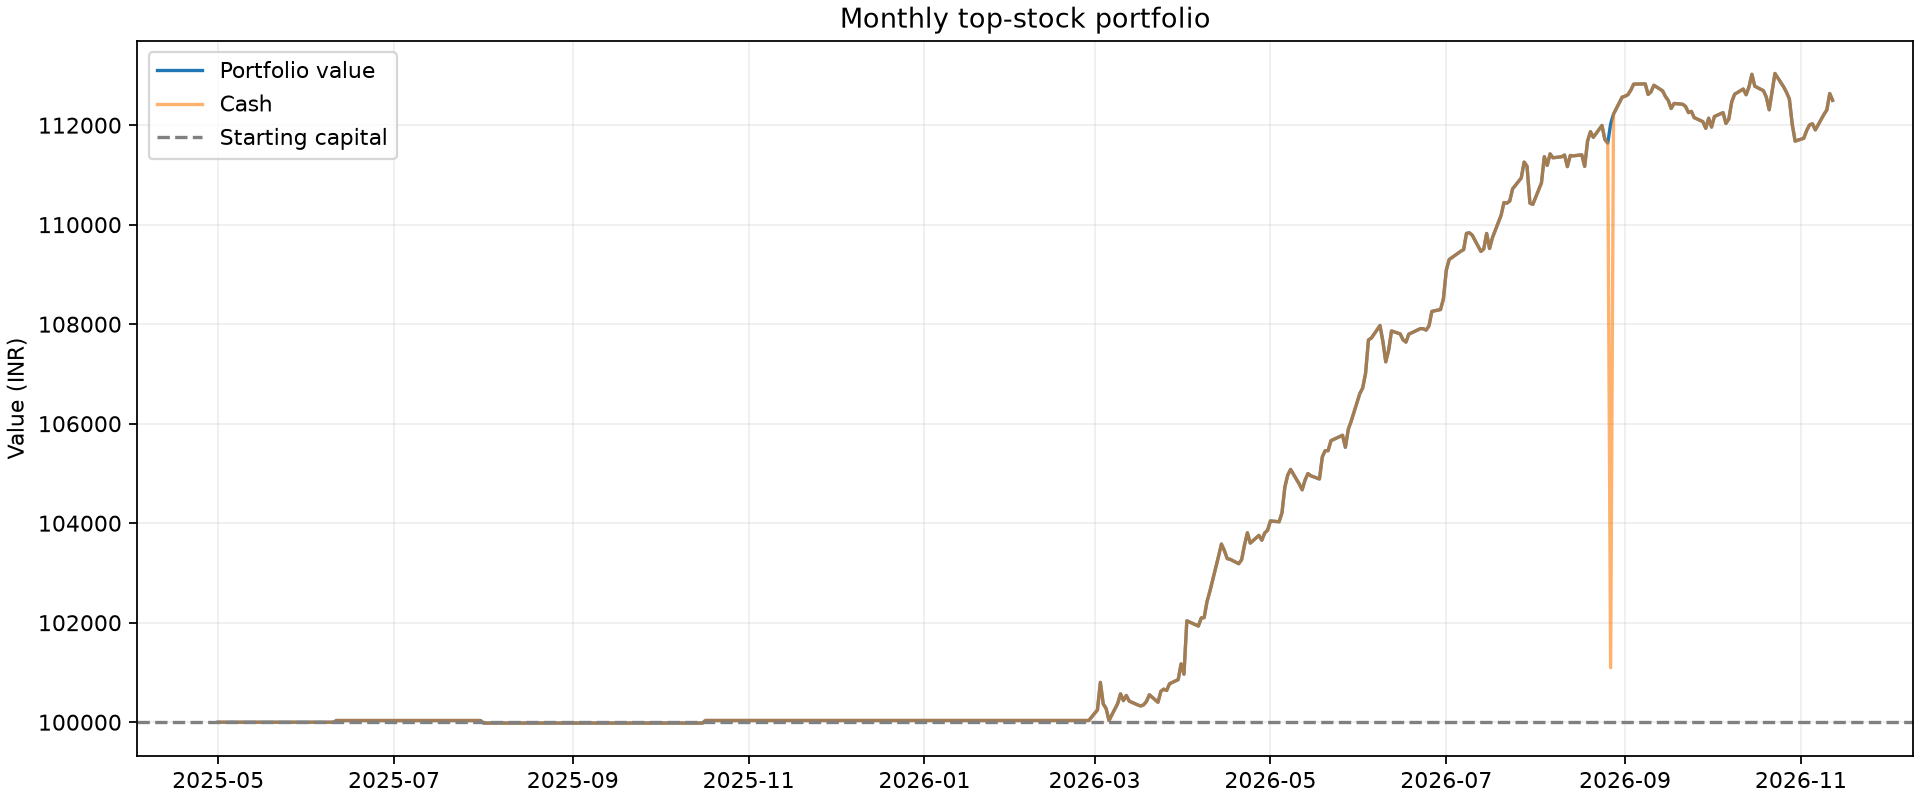
\includegraphics[width=\linewidth,height=4.45cm,keepaspectratio]{11-portfolio_value.png}
\par\smallskip{\small 1 May 2025--12 November 2026 \qquad USD 100,000 to USD 112,499.25 \qquad \textbf{+12.50\%}}
\note{\textbf{10:53 to 11:05}\par The US top-20 account grew from USD 100,000 to about USD 112,499. A rising equity curve looks promising in isolation. The next slide supplies the missing comparison.}
\end{frame}

\begin{frame}{US portfolios traded sparsely and trailed holding}
\pair{monthly-us.png}{May 2025--November 2026}{Top 10 gained \textbf{8.92\%} and top 20 gained \textbf{12.50\%}. Equal-money buy-and-hold gained \textbf{40.97\%}.\\[2mm]
Only one stock had a trailing score before March 2026. Even over the active period, top 20 gained 12.46\% against 13.28\% for holding.}
\note{\textbf{11:05 to 11:47}\par Over the same US period, holding earned 40.97 percent, well above the top-20 strategy's 12.50 percent. Only one stock had a trailing score before March 2026, so initially there was little opportunity to deploy capital. Even over the active period, top 20 earned 12.46 percent against 13.28 percent for holding. Sparse trading explains part of the story; exposure-matched testing would help quantify it.}
\end{frame}

\begin{frame}{Fees absorbed over half of India's top-10 trading profit}
\centering
{\small Each bar represents 100\% of its top-10 portfolio's profit before recorded fees.}\par\medskip
\begin{tikzpicture}[x=.113cm,y=1cm,font=\small]
\foreach \y/\fee/\net/\market/\amounts in {
  1.55/57.68/42.32/India/{INR 3,419,384 in fees; INR 2,508,725 retained},
  0/12.52/87.48/US/{USD 1,277 in fees; USD 8,923 retained}}{
  \node[anchor=east,font=\bfseries] at (-2,\y+.25) {\market};
  \fill[iitiblue] (0,\y) rectangle (\fee,\y+.5);
  \fill[iiticyan!17] (\fee,\y) rectangle (100,\y+.5);
  \node[text=white] at (\fee/2,\y+.25) {\fee\%};
  \node[text=iitiblue] at ({(100+\fee)/2},\y+.25) {\net\%};
  \node[anchor=north west,inner xsep=0pt,font=\footnotesize] at (0,\y-.04) {\amounts};}
\end{tikzpicture}\par\smallskip
{\footnotesize\textcolor{iitiblue}{$\blacksquare$} Recorded fees\qquad\textcolor{iiticyan!35}{$\blacksquare$} Profit retained}\par\medskip
\raggedright\small Covering recorded charges took about \textbf{5.21 basis points} per round trip in India and \textbf{0.29} in the US replay under its zero-commission assumption.
\note{\textbf{11:47 to 12:31}\par Each bar is one portfolio's gross trading profit. The dark segment is the part spent on recorded fees. India used about 58 of every 100 rupees of pre-fee profit; the US replay used about 13 of every 100 dollars. Those are shares of profit, not fee rates per transaction. The US replay assumes zero commission. Differences in trades, dates, sizing and brokerage assumptions limit the cross-market comparison.}
\end{frame}

\begin{frame}{How did the RL agent choose a trade?}
\begin{columns}[T,onlytextwidth]
\begin{column}{.48\textwidth}
\begin{block}{Observe each stock: 13 inputs}
\small\textbf{4 prices:} open, high, low and close relative to the previous close.\\[2pt]
\textbf{5 signals:} VWAP, RSI, Bollinger, Donchian and the evolved entry rule.\\[2pt]
\textbf{4 account/time inputs:} holding flag, position weight, cash fraction and time of day.
\end{block}
\end{column}
\begin{column}{.49\textwidth}
\begin{block}{Act in a simulated US trading account}
\small Each minute, choose \textbf{hold, buy or sell} for each of 95 stocks. Eligible orders fill at the next bar's open.\\[3pt]
Start with USD 100,000. Allocate about 4\% per entry, hold up to 10 long positions and close positions near session end.
\end{block}
\end{column}
\end{columns}
\smallskip\centering
$ r_t=\log(E_t/E_{t-1})-\max(0,D_t-D_{t-1}) $\par
\small One reward for the whole account: growth in equity $E$ after fees, with a penalty whenever drawdown $D$ deepens.
\note{\textbf{12:31 to 13:08}\par Imagine the first minute of trading. For each stock the agent sees four price changes, five strategy signals and four account or time inputs. It chooses hold, buy or sell. All stocks compete for ten slots in one account, and eligible orders execute at the next open. The reward measures account growth after fees. If the portfolio falls farther below its previous peak, the reward takes an extra penalty. A flat minute adds no further penalty.}
\end{frame}

\begin{frame}{A drawdown-aware policy gained 4.02\% on held-out data}
\pair{12-equity.png}{US test: 1 September--12 November 2026}{The saved account grew from USD 100,000 to \textbf{USD 104,016.35} after USD 57.03 in fees. Maximum drawdown was \textbf{1.38\%}.\\[2mm]
All 520 buys filled at \textbf{09:31 New York time}. The median holding time was 384 minutes.}
\note{\textbf{13:08 to 13:38}\par The saved run gained 4.02 percent. The trades tell us what the policy actually did: it bought at 09:31 and usually held until near the close. The simulator imposed end-of-session liquidation. The original input cache is missing; replaying the checkpoint on a later cache returned 3.74 percent. The five signals were inputs, but their contribution to the gain remains uncertain.}
\end{frame}

\section{Conclusion}
\subsection*{}
\begin{frame}{What the experiments establish}
\small
\begin{block}{Forecasting}
USD/INR's 55.51\% directional accuracy translated into three extra correct days over always-up. A repeated-seed comparison with standard squared error would isolate the contribution of loss design.
\end{block}
\begin{block}{Execution}
EUR/USD earned a positive return with more losses than wins. Finer price data would help test which stops and targets could actually have filled.
\end{block}
\begin{block}{Portfolio performance}
The Indian top 10 beat holding after recorded fees. Both US portfolios trailed their benchmark. Testing on new periods with matched exposure would help distinguish signal quality from time spent invested.
\end{block}
\note{\textbf{13:38 to 14:21}\par Three results summarize my project. First, 55.51 percent accuracy translated into only three extra USD/INR calls. Second, the EUR/USD simulation made money with more losing trades than winners because payoff sizes differed. Third, the Indian top 10 beat holding after fees while both US portfolios trailed it. My next experiment would freeze the rules, test a new period and match market exposure. Thank you. I welcome your questions.}
\end{frame}

\section{Appendix}
\subsection*{}
\begin{frame}{Appendix A: From market data to features}
\centering
\begin{tikzpicture}[workflow/.style={draw=iitiblue!35,fill=iitilightbg,rounded corners=2pt,text width=6.45cm,inner sep=3pt,align=left,font=\small},link/.style={->,draw=iiticyan,thick}]
\node[font=\bfseries,text=iitiblue] at (0.0,0) {Daily forex};
\node[workflow,minimum height=1.32cm] (w00) at (0.0,-1.00) {\textbf{Data}\\ Daily exchange rates and US interest rates.};
\node[workflow,minimum height=1.32cm] (w01) at (0.0,-2.65) {\textbf{Preprocessing}\\ Align dates, calculate log returns and fit scaling on training data.};
\draw[link] (w00.south) -- (w01.north);
\node[workflow,minimum height=1.32cm] (w02) at (0.0,-4.30) {\textbf{Features}\\ Build 23 currency, rate and technical features.};
\draw[link] (w01.south) -- (w02.north);
\node[font=\bfseries,text=iitiblue] at (7.25,0) {Intraday equities};
\node[workflow,minimum height=1.32cm] (w10) at (7.25,-1.00) {\textbf{Data}\\ Minute bars for 100 Indian and 95 US stocks.};
\node[workflow,minimum height=1.32cm] (w11) at (7.25,-2.65) {\textbf{Preprocessing}\\ Audit missing minutes. Restart rolling windows after gaps and at session boundaries.};
\draw[link] (w10.south) -- (w11.north);
\node[workflow,minimum height=1.32cm] (w12) at (7.25,-4.30) {\textbf{Features}\\ Screen 61 NIFTY indicators. Retain 32 after removing price levels and redundant features.};
\draw[link] (w11.south) -- (w12.north);
\end{tikzpicture}
\note{\textbf{Q\&A only}\par Use if asked where the two tracks diverge. On the left, align daily macro and FX observations and fit the scaler on training data. On the right, audit minute bars, restart at gaps and session boundaries, and build intraday features. The 23 forex inputs and 32 screened equity indicators belong to different experiments.}
\end{frame}
\begin{frame}{Appendix A: From models to portfolios}
\centering
\begin{tikzpicture}[workflow/.style={draw=iitiblue!35,fill=iitilightbg,rounded corners=2pt,text width=6.45cm,inner sep=3pt,align=left,font=\small},link/.style={->,draw=iiticyan,thick}]
\node[font=\bfseries,text=iitiblue] at (0.0,0) {Daily forex};
\node[workflow,minimum height=1.32cm] (w00) at (0.0,-1.00) {\textbf{Models}\\ Predict next-day returns with a 32-unit LSTM and magnitude-weighted loss.};
\node[workflow,minimum height=1.32cm] (w01) at (0.0,-2.65) {\textbf{Execution}\\ Tune entries, stops, targets and sizing. Simulate EUR/USD execution.};
\draw[link] (w00.south) -- (w01.north);
\node[workflow,minimum height=1.32cm] (w02) at (0.0,-4.30) {\textbf{Evaluation}\\ Compare strategy and passive returns over the same 65 sessions.};
\draw[link] (w01.south) -- (w02.north);
\node[font=\bfseries,text=iitiblue] at (7.25,0) {Intraday equities};
\node[workflow,minimum height=1.32cm] (w10) at (7.25,-1.00) {\textbf{Models}\\ Test intraday forecasts, optimize strategy parameters and evolve entry-rule trees.};
\node[workflow,minimum height=1.32cm] (w11) at (7.25,-2.65) {\textbf{Execution}\\ Apply shared-capital limits and charge fees on executed orders.};
\draw[link] (w10.south) -- (w11.north);
\node[workflow,minimum height=1.32cm] (w12) at (7.25,-4.30) {\textbf{Evaluation}\\ Evaluate top-10 and top-20 portfolios. Pass five signals to the intraday RL policy.};
\draw[link] (w11.south) -- (w12.north);
\end{tikzpicture}
\note{\textbf{Q\&A only}\par Trace just the column relevant to the question. Forex goes from next-day return prediction to a EUR/USD execution replay. Equities go from signals and rule search to a shared account, fees and portfolio evaluation. The RL policy is a further experiment with its own test period.}
\end{frame}
\begin{frame}{Can a repaired minute leak future prices?}
\begin{block}{Where leakage could enter}
ABB, 13 March 2015. The historical repair uses prices on both sides of a gap. Using the repaired 09:27 bar at 09:27 would reveal a later price.
\end{block}
\begin{block}{What the forecasting loader does}
Discard repaired bars, recalculate indicators from observed prices and keep each 30-minute input and next-minute target in one continuous segment. Split whole sessions chronologically.
\end{block}
\begin{block}{What the check established}
Clearing all eight repaired bars left all 278 eligible input windows, target timestamps and returns identical. The check covers one ABB session and the current forecasting loader.
\end{block}
\note{\textbf{Q\&A only}\par Yes. A two-sided repair uses later prices. The current forecasting loader discards repaired bars and recalculates features from observed prices. For ABB on 13 March 2015, clearing all eight repaired bars left all 278 eligible windows, target timestamps and target returns identical. This directly tests one leakage pathway in one session. Extending it requires checking other symbols, periods and loaders.}
\end{frame}
\begin{frame}{How did the actor and critic learn?}
\small
\begin{block}{One shared network, two outputs}
For each stock: $13\to64\to64$ with tanh activations. The \textbf{actor} scores hold, buy and sell. The \textbf{critic} gives one value per stock; averaging all 95 gives the expected portfolio reward.
\end{block}
\begin{block}{Learning from a rollout}
Sample actions for up to 256 minutes. The advantage is discounted reward target minus predicted value ($\gamma=0.99$). The loss combines actor loss, $0.5\times$ critic squared error and a $0.001$ entropy bonus for exploration. Adam learning rate: $0.0003$.
\end{block}
\begin{block}{Evaluation}
Train Dec 2025--May 2026. Select among five epochs on June--August return minus maximum drawdown magnitude. On the later test, take each stock's most probable valid action. Buy probability ranks competing entries.
\end{block}
\note{\textbf{Q\&A only}\par The same two-layer network processes each stock. Its actor produces action probabilities; its critic estimates a baseline used during training. At test time the actor alone determines the requested actions. During training a positive advantage reinforces the sampled portfolio decisions; the critic learns to predict the discounted target. The trainer scales step rewards by 100. Drawdown is one minus equity divided by peak equity. For example, a fall from 100,000 to 99,900 at a new peak produces roughly -0.001 log growth and -0.001 drawdown penalty, or -0.002 before scaling.}
\end{frame}
\end{document}

